\section{Results}
\subsection{Polyploidy and Diversification Models}
Similarly to the results obtained by \citet{mayrose_2011} and \citet{mayrose_2015}, we found that in the D/P polyploidy model the net diversification of diploids is larger than the the net diversification of polyploids since the net diversification distributions do not overlap (Figure 2(A)). This result holds true whether or not the diploidization parameter is present. However in the presence of  the diploidization parameter the net diversification rate of polyploids is nonnegative with probability 1 (Figure 2(A)), whereas in the absence of diploidization the net diversification rate of polyploids can be negative with a probability (HERE verify the quantile) (FIGURE 3(A)). In terms of the relative extinction, when the diploidization parameter is present both polyploids and diploids have posterior distributions that overlap, but that pattern changes in the absence of the diploidization parameter leading to a significant difference between relative extinction where polyploids have a significant higher relative extinction rate (see Supplementary Information).\newline

For the D/P- A/B model with diploididization the diploid and polyploid net diversification rates are overlapping for both state A and B of the hidden trait (Figure 2(B)). In this model, the differences in net diversification are due to the presence of a hidden trait and not to the differences in ploidy. When diploidization parameter is absent the hidden state is still driving the differences in diversification rates (Figure 3(B)).



\subsection{Breeding System and Diversification models }
In the I/C breedyng system model we found that the net diversification rate for self-incompatible state is larger than the net diversification rate for self-compatible state (Figure 2(C)). The net diversification rate for self-compatible has a probability distribution centered at zero.  \newline

When a hidden state is added in the I/C-A/B model, we found that under the hidden state A the self-compatible and self-incompatible net diversification rates are different. Under the hidden state B, those two rates overlap with a probability (HERE CALCULATE THAT) meaning that they are different with probability  (CALCULATE) (Figure 2(D)). These results agree with previous results found by  \citet{goldberg_2012}. However, \citet{goldberg_2012} used a ClaSSE  approach since they were interested in anagenetic and cladogenetic changes for self-incompatibility using a smaller subset of the data presented in the current work.

% Describe rate q_IC and hidden state rate

\subsection{Polyploidy and Breeding Sytem models}
In the ID/P/CD model we found that self-incompatible and diploid state has a significantly larger net diversification rate compare to both self-compatible diploid and polyploid rates. Meanwhile, both self-compatible diploid and polyploid posterior distributions of net diversification rates completely overlap (Figure 2(E)). When hidden state was added in the ID/P/CD-A/B model, we observed significant differences between self-compatible and self-incompatible diploids for both A and B values of the hidden state. Self-incompatible state had a larger net diversification rate than self compatible for both A and B states. However, the posterior distribution for the net diversification rate of polyploids overlaps with both the self-compatible and self-incompatible posterior distributions for each value of the hidden state(Figure 2F) meaning that polyploidy state is not significantly different from diploid in net diversification terms.  The resulting effect of adding the hidden state values is significant 


\subsection{Diploidization as an exploratory hypothesis}
In the D/P model  the diploidization rate $\delta$ and polyploidization rate $\rho$ are different from zero with probability 1. Diploidization rate is more uncertain than polyploidization. For the D/p no $\delta$ model, the polyploidization rate is still different from zero but has a wider 95\% credible interval (see Supplementary Information).

For the models containing both polyploidy and breeding system traits, we found that the diploidization rate is really uncertain with a MAP that is (CALCULATE VALUE HERE- close to zero). The polyploidization rate from self-incompatible diploid $\rho_I$ is slightly faster than the polyploidization rate from self-compatible diploid $\rho_C$






\begin{figure}
\centering
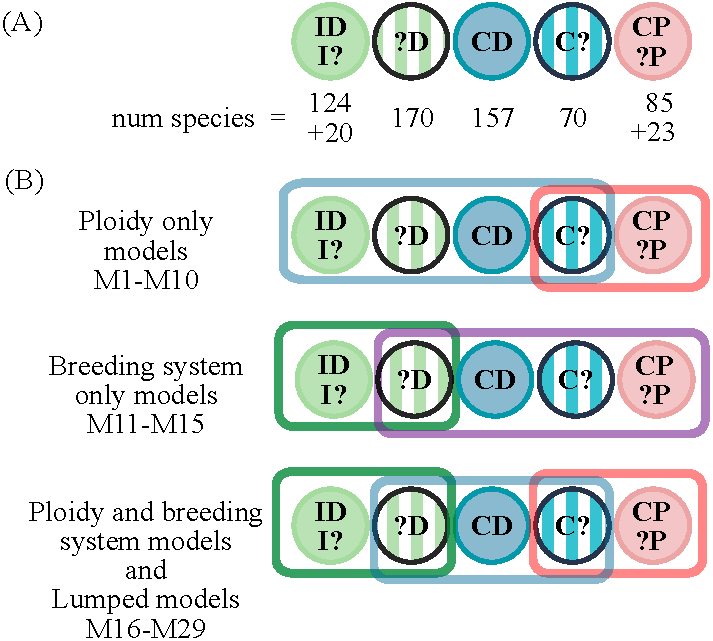
\includegraphics[width=0.5\textwidth]{states.pdf}
  \caption{Binary and three state classifications for 595 taxa with ploidy and/or breeding system data. The number of taxa in the the sample was maximized by including tips with only ploidy or only breeding system and assigned them as uncertain in some of the models. For example, the 34 self-compatible taxa with unknown ploidy were assigned as uncertain (diploid or polyploid) in the D/P models but as fully compatible in the I/C models.}  
\label{figure:stateclassifications}
\end{figure}


\begin{figure}
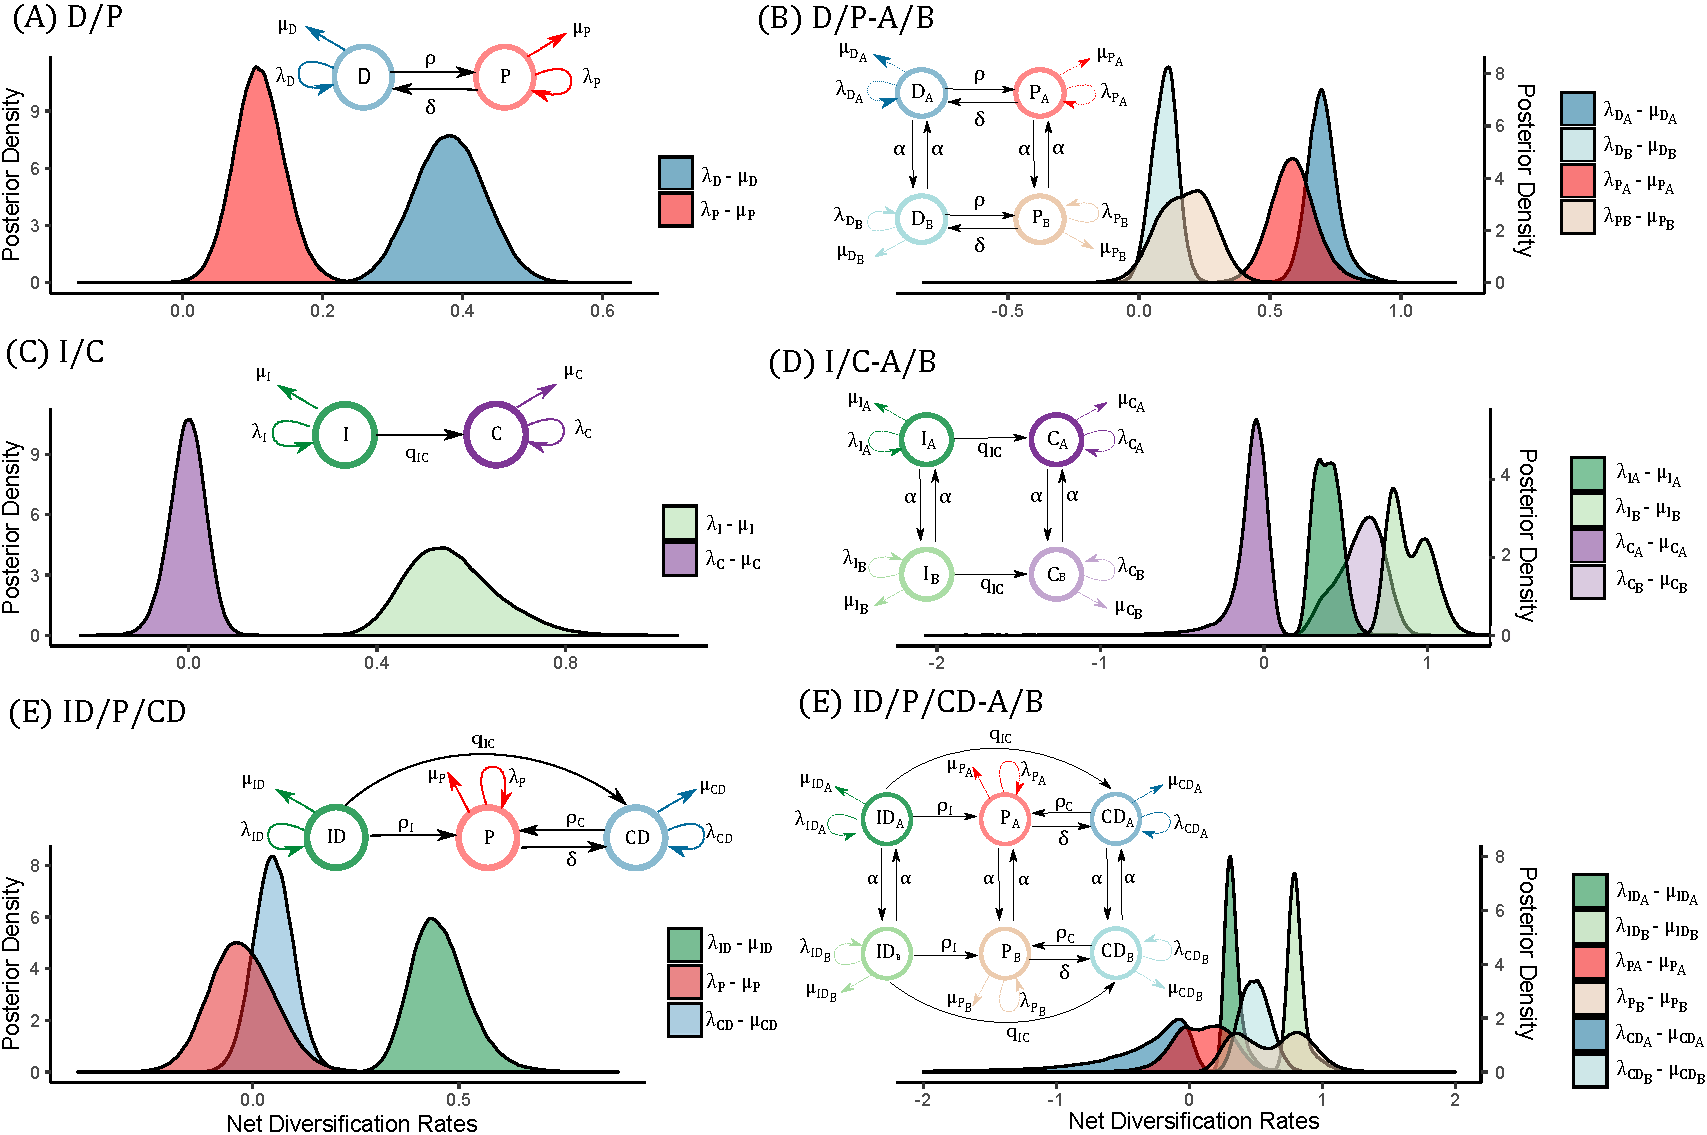
\includegraphics[width=\textwidth]{Netdiversificationallmodels.pdf}
  \caption{Net diversification rates for all models that include diploidization.}  
\label{figure:netdivall}
\end{figure}